\chapter{Doug Williams: Focus, Scale, and the Risk Meter}

This chapter follows a School of Hard Knocks entrepreneurship interview, curated by LazyingArt LLC with Video2Book. The source is not a blackboard derivation, but it does have a quantitative spine. Doug Williams moves from capital allocation to operating focus, from selling to scaling, and then from career durability to risk judgment. The numbers are few and therefore worth preserving: a $50$ million venture pool, early checks of roughly $500{,}000$ to $2$--$3$ million, portfolio companies often below $2$ million in revenue, five and a half million American miles, and an HMS Holdings sale reported at $3.5$ billion. We will use those numbers as anchors while keeping the main lesson in view: entrepreneurship is a sequence of judgments about focus, credibility, preparation, alignment, and risk.

\section{Credentials, Capital, and the Investor's Filter}

The interview opens by establishing scale. Williams is introduced as the former chief operating officer of HMS Holdings, a healthcare company sold for about
\begin{equation}
V_{\mathrm{exit}} \approx \$3.5\text{ billion}.
\end{equation}
That opening is not merely biographical. It tells us what kind of evidence the chapter is built from: operating experience, board work, healthcare markets, sales into large organizations, and venture investing.

The first real question asks what he looks for in a company. Williams answers in the order an investor actually feels the problem: first capital, then stage, then quality. The investment vehicle has about
\begin{equation}
C \approx \$50{,}000{,}000
\end{equation}
available to invest. It participates in early rounds, and the typical check is somewhere in the range
\begin{equation}
I \in [\$500{,}000,\ \$2{,}000{,}000\text{ to }\$3{,}000{,}000].
\end{equation}
The companies are not yet mature machines. Williams says they are often generating less than roughly
\begin{equation}
R \lesssim \$2{,}000{,}000
\end{equation}
in revenue.

Now the qualitative filter makes sense. At that stage, Williams looks for interesting ideas, thoughtful management teams, and large target markets. Those criteria are not ornamental. A weak idea cannot carry early uncertainty; an unthoughtful team cannot process advice; and a small market limits the payoff even if execution improves.

A compact reconstruction of the investment filter is
\begin{equation}
\text{investable company}
\approx
\text{idea}
+
\text{team}
+
\text{market}
+
\text{focus}.
\end{equation}
This is not a formula from a board. It is a concise notation for the order of his answer. The money enters only after the company has enough raw material for coaching to matter.

\paragraph{A small scale calculation.}
If every check were at the low end, \(I=\$500{,}000\), then a \(C=\$50{,}000{,}000\) pool could theoretically write
\begin{equation}
N_{\max}=\frac{C}{I}
=
\frac{50{,}000{,}000}{500{,}000}
=
100
\end{equation}
such checks before reserves and follow-on capital. If every check were closer to \(I=\$2{,}500{,}000\), the same pool would support about
\begin{equation}
N \approx \frac{50{,}000{,}000}{2{,}500{,}000}=20
\end{equation}
checks. The interview does not say this is the fund construction. The calculation simply makes the scale concrete: early-stage investing is a portfolio problem, but each company still requires concentrated operating attention.

\section{Focus as the Investor's Operating Role}

Williams then moves from what he funds to what he does after funding. Young CEOs, he says, can have too many things coming at them and too few people to handle them. The central operating difficulty is not only scarcity of money. It is scarcity of attention.

He describes his role as coaching CEOs, direct reports, and boards toward the right target. The sectors he names are behavioral health and digital health, including concussion monitors, anxiety-related work for troops, and drug studies. The examples vary, but the operating problem has the same shape: a young company must decide which actions actually move the business.

Let \(A\) denote the set of actions confronting a CEO. Most of \(A\) is noise, distraction, or work that is real but not decisive. The board member and investor are trying to help identify a smaller set,
\begin{equation}
A^\ast
=
\{a \in A:\ a \text{ is focused, timely, and material}\}.
\end{equation}
The movement from \(A\) to \(A^\ast\) is one of the chapter's main mechanisms. Focus is not a slogan here; it is a compression of the action space.

\begin{figure}
\centering
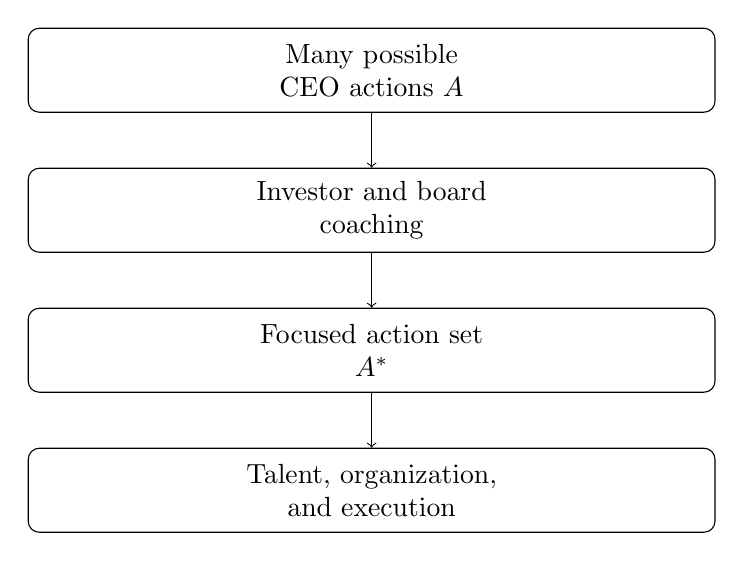
\begin{tikzpicture}[
  box/.style={draw, rounded corners, align=center, text width=0.70\linewidth, minimum height=0.42in},
  node distance=0.70in
]
\node[box] (a) {Many possible\\CEO actions \(A\)};
\node[box, below of=a] (b) {Investor and board\\coaching};
\node[box, below of=b] (c) {Focused action set\\\(A^\ast\)};
\node[box, below of=c] (d) {Talent, organization,\\and execution};
\draw[->] (a) -- (b);
\draw[->] (b) -- (c);
\draw[->] (c) -- (d);
\end{tikzpicture}
\caption{Transcript-backed reconstruction of the investor's role as a focus mechanism.}
\end{figure}

\section{Selling Through Consequence, Not Hype}

The interviewer next asks for a coaching example. Williams describes a founder who was smart, knew the market, and understood the product, but whose message was not going to land. The failure point was not intelligence. It was translation into buyer consequence.

His phrase is that one sells through fear, not foresight. We should read that carefully. He is not recommending panic or deception. He is saying that a buyer often reacts more concretely to the cost of failure than to an abstract promise of success. A CEO does not wake up afraid of too much success. The CEO worries about what will break, what will be exposed, and what will hurt the business if left unsolved.

\subsection{Question \& Answer}

\paragraph{Question.}
Why emphasize fear of failure rather than the upside of success?

\paragraph{Answer.}
Because the buyer's immediate problem is usually not a vague future benefit. It is a present vulnerability. If the seller can show, truthfully and specifically, that ignoring the issue will damage the buyer's business, the buyer has a reason to act. The message becomes: this is the failure you avoid by solving the problem now.

Williams then adds a second ingredient: credibility. A small company selling into a large company faces a scale gap. In his example, a company near $2$ million in size may be selling to a $50$ billion company. The inequality is the point:
\begin{equation}
\text{seller scale} \ll \text{buyer scale}.
\end{equation}
The buyer may like the idea but still distrust the capacity of the seller. Williams's market credibility can reduce that gap. If the buyer trusts him, some of that trust can transfer to the company he brings forward. But the trust was not produced by the transaction; it was accumulated over years.

The three measures he wants CEOs to focus on are message, relevance to the buyer, and unique differentiation. In notation, the sales claim has to answer
\begin{equation}
\text{Why this problem?}
\qquad
\text{Why this buyer?}
\qquad
\text{Why this company?}
\end{equation}
If any one of those is vague, the sales motion loses force.

\section{Solution Selling: Let the Buyer Buy}

The next question makes the sales theme explicit: how does someone crush sales? Williams begins with a distinction that governs the whole answer: no one likes to be sold to, but everybody likes to buy. Selling is therefore not a performance in which the seller shows everything and hopes the buyer reacts. It is a diagnostic sequence.

The sequence is deliberate:
\begin{enumerate}
\item do homework before the meeting;
\item ask questions before showing the product;
\item understand the real need;
\item identify the buyer's pain points;
\item solve the problem mutually.
\end{enumerate}
This reverses the demo-first habit. In the weak version, the seller says: here is everything we have, stop me when something interests you. In Williams's version, the seller starts by understanding the buyer's state.

A concise update rule for the conversation is
\begin{align}
\text{homework}
&\longrightarrow
\text{questions},\\
\text{questions}
&\longrightarrow
\text{true need},\\
\text{true need}
&\longrightarrow
\text{pain point},\\
\text{pain point}
&\longrightarrow
\text{mutual solution}.
\end{align}
The important word is ``mutual.'' The seller is not simply pushing inventory. The seller is making the buyer's own decision legible.

\begin{figure}
\centering
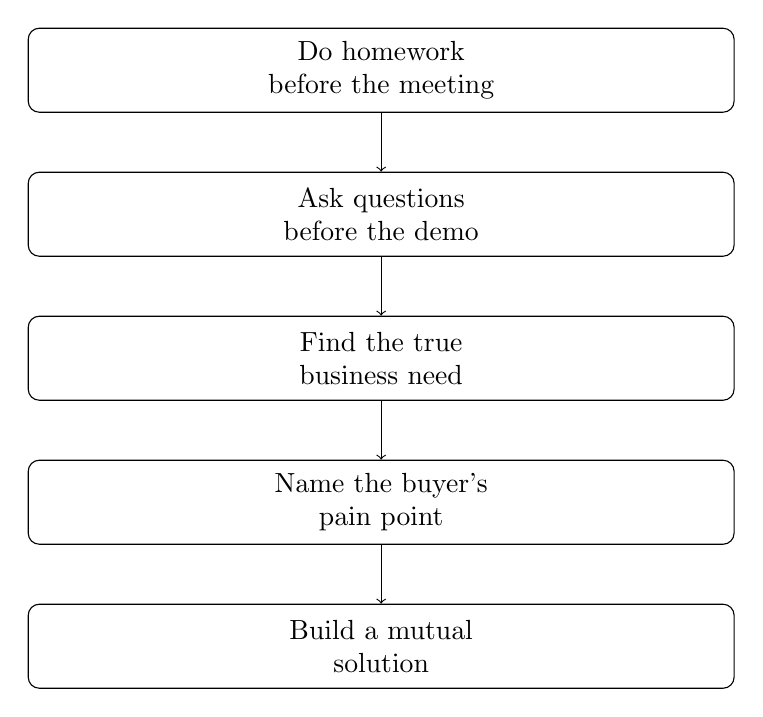
\begin{tikzpicture}[
  box/.style={draw, rounded corners, align=center, text width=0.72\linewidth, minimum height=0.42in},
  node distance=0.72in
]
\node[box] (a) {Do homework\\before the meeting};
\node[box, below of=a] (b) {Ask questions\\before the demo};
\node[box, below of=b] (c) {Find the true\\business need};
\node[box, below of=c] (d) {Name the buyer's\\pain point};
\node[box, below of=d] (e) {Build a mutual\\solution};
\draw[->] (a) -- (b);
\draw[->] (b) -- (c);
\draw[->] (c) -- (d);
\draw[->] (d) -- (e);
\end{tikzpicture}
\caption{Transcript-backed reconstruction of Williams's solution-selling sequence.}
\end{figure}

\section{Scaling as a Designed Doubling Playbook}

The interviewer then asks how a business scales from six figures to seven, eight, and toward the scale of the HMS sale. Williams first gives the standard valuation language: companies are often sold from a multiple of revenue or EBITDA. Since no multiple is given, the safe form is only a shorthand:
\begin{equation}
V \approx m_R R
\qquad\text{or}\qquad
V \approx m_E E,
\end{equation}
where \(R\) is revenue, \(E\) is EBITDA, and \(m_R,m_E\) are unspecified market multiples. We should not derive the HMS transaction from this equation. The transcript only reports the sale value.

The operating answer comes next. To move a company to scale, Williams says to get the basics right: value proposition, total addressable market, buyer, and key message. Only then does the wheel start to spin. Once it spins, the company must not improvise every stage of growth.

His image is a folding piece of paper. Plan the company where it is today. Then ask what happens when it doubles. Then ask again. If \(S_0\) is the present scale, the reconstructed doubling model is
\begin{equation}
S_n = 2^nS_0.
\end{equation}
This is not a literal board equation. It is the mathematical skeleton of the verbal model.

\subsection{Question \& Answer}

\paragraph{Question.}
What has to be designed before a company scales?

\paragraph{Answer.}
Not just the product, and not just the next sales push. Williams names organizational structure, metrics, alignment, relationships, and channels. These are the operating rails that let the next doubling happen with less wasted motion.

\begin{figure}
\centering
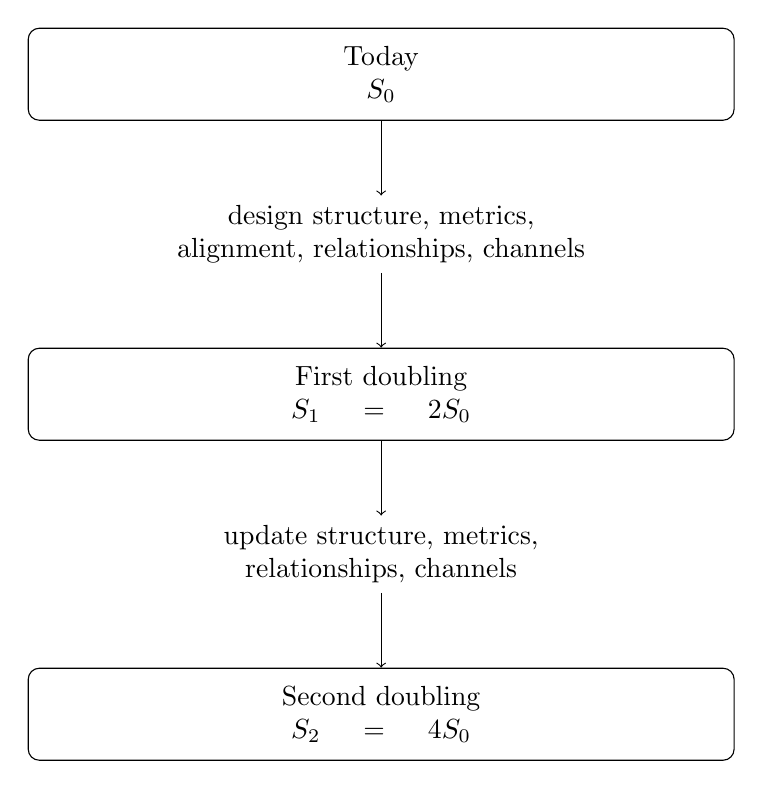
\begin{tikzpicture}[
  stage/.style={draw, rounded corners, align=center, text width=0.72\linewidth, minimum height=0.46in},
  small/.style={align=center, text width=0.72\linewidth},
  node distance=0.80in
]
\node[stage] (s0) {Today\\\(S_0\)};
\node[small, below of=s0] (p0) {design structure, metrics,\\alignment, relationships, channels};
\node[stage, below of=p0] (s1) {First doubling\\\(S_1=2S_0\)};
\node[small, below of=s1] (p1) {update structure, metrics,\\relationships, channels};
\node[stage, below of=p1] (s2) {Second doubling\\\(S_2=4S_0\)};
\draw[->] (s0) -- (p0);
\draw[->] (p0) -- (s1);
\draw[->] (s1) -- (p1);
\draw[->] (p1) -- (s2);
\end{tikzpicture}
\caption{A transcript-backed reconstruction of scaling by planned doublings.}
\end{figure}

The payoff is speed. If the next version of the organization is already imagined, raising money, using a banking relationship, or adding leverage has a frame around it. Scaling by design is faster than simply trying to do more and more of the same thing.

\section{Career Durability and the Cost of Money Alone}

The lecture then changes register without leaving the theme. Williams discusses his book, \emph{Shift: A Playbook for Positive Change}, whose working title was closer to \emph{Enjoy the Walk} or \emph{Enjoy the Journey}. The important lesson is not the book title. It is the idea that a career is built out of skills learned and people met, not only jobs held.

This widens the notion of entrepreneurship. The company matters, the job matters, and the exit matters, but Williams keeps returning to mentors, colleagues, and helping people move up. Even when someone changes career or leaves one's direct orbit, helping that person improve is part of the long-run network. The mechanism is practical: durable careers are built inside relationships.

The question of work-life balance makes the same point in a sharper form. Williams says it was always front of mind. He also gives the scale of his travel:
\begin{equation}
M_{\mathrm{travel}} \approx 5.5\text{ million miles}.
\end{equation}
His rule was contextual. When away from the family, he worked. When home, he was home:
\begin{equation}
\text{away} \mapsto \text{work},
\qquad
\text{home} \mapsto \text{family}.
\end{equation}
He avoided calls all day Saturday. On Sunday night, after everyone went to bed, he might spend an hour or an hour and a half preparing for the week.

The warning that follows is one of the interview's plainest claims. A person can work intensely, retire with money, and discover that the relationships, friendships, and family ties were not built. Money alone is not the durable end state. It is purchasing power without the human structure that makes it enjoyable.

\section{Mental Balance and Transferable Skill}

The mental-health question continues the same logic at the level of daily practice. Williams says one must have more than one focus in life. His rhythm is specific: up at 4:30, in the gym by 5, generally working out seven days a week. Some days include more than one workout. Exercise is not only physical maintenance; it is mind space.

The hobbies are part of the same operating system: golf, sailing, hiking, and road biking. The Abraham Lincoln sharpening-the-ax anecdote gives the principle its simplest form. Recovery and renewal are not interruptions of productive work. They are part of the preparation that makes productive work possible.

Then the interview returns to career history. Williams began as a computer programmer. In his first job he programmed devices, worked on B-1 bombers, worked on Disneyland systems, and learned how devices communicate. The transferable skill was not merely coding. It was working with protocols, companies, users, and field problems.

That field exposure led to Arthur Andersen, where he became a partner, then healthcare technology leadership, healthcare IBM consulting worldwide, and finally HMS Holdings. The path can be written as a compounding chain:
\begin{equation}
\text{programming}
\longrightarrow
\text{field devices}
\longrightarrow
\text{protocols and people}
\longrightarrow
\text{consulting}
\longrightarrow
\text{healthcare operations}
\longrightarrow
\text{HMS}.
\end{equation}
The opening credential now appears as the result of a sequence, not an isolated title. Technical ability became commercial judgment because it was repeatedly tested against real systems and real organizations.

\section{Risk, Due Diligence, and Helping Others}

The final movement begins with financial decisions. Williams jokes that his worst decision was not buying enough Bitcoin or Tesla. More seriously, he says he has lost money on one investment, but when he reviewed the data and the people he was betting on at the time, he still thought it was a good bet. That distinction is important: a bad outcome is not automatically a bad decision.

The risk principle is qualitative:
\begin{equation}
\text{perfect success rate}
\quad\Rightarrow\quad
\text{risk meter may be too low}.
\end{equation}
This is not expected-value mathematics, and the transcript does not support a probability model. It is an operating warning. If every investment works, perhaps the investor is not taking enough uncertainty to find exceptional outcomes.

Williams's due-diligence rule is to know people before investing with them. Not merely through a demo or a PowerPoint presentation. Meet them, talk to them, get offline, and understand character. The reason is simple: no business plan goes off flawlessly. When the plan breaks, the people remain.

A narrow reconstruction of the due-diligence ladder is
\begin{equation}
\text{deck}
\longrightarrow
\text{conversation}
\longrightarrow
\text{context}
\longrightarrow
\text{character}
\longrightarrow
\text{alignment}.
\end{equation}
The last word is the strongest. On boards, and among people brought in to help companies, Williams wants shared respect and a shared goal. The objective is to make the play successful, not to be the brightest light in the room.

The closing advice to Gen Z completes the chapter's pattern. Ask what you can do to help, not merely what you can do to get ahead. Look for situations where you can lift somebody else up. The commercial mechanism is accumulated trust. The human mechanism is just as important: if one builds a career alone, one should not be surprised to end up alone.

\section{Summary}

The lecture's center of gravity is disciplined judgment. Williams begins with capital, but capital alone is not the lesson. Early-stage investing requires a filter: idea, team, market, stage, focus, and talent. Selling requires diagnosis rather than performance. Scaling requires a staged doubling playbook. Career durability requires relationships, family boundaries, health, and renewal. Risk requires enough uncertainty to matter, and enough due diligence to know the people taking the risk with you.

The mathematical frame is modest because the source is an interview, not a board lecture. Still, the quantities organize the chapter: \(C \approx \$50{,}000{,}000\), early checks \(I\) around $500{,}000$ to $2$--$3$ million, revenue stage \(R \lesssim \$2{,}000{,}000\), valuation shorthand \(V \approx m_RR\) or \(V \approx m_EE\), and staged scale \(S_n=2^nS_0\). These symbols are useful only when they serve the underlying claim: entrepreneurship is growth under focus, credibility, preparation, alignment, and risk fit.